% !TeX program = xelatex
\documentclass[a4paper,12pt]{article}

\usepackage{tabularx}
\usepackage[font=small,labelfont=bf]{caption}
\usepackage{graphicx}
\usepackage[localise=on]{xepersian}

\settextfont{B Zar}
\linespread{1.25}

\title{گزارش پروژه سوم درس داده‌کاوی}

\author{
پرهام کاظمی \\ ۹۴۳۶۱۱۰۴۳۰۱۸
\and
علیرضا پرچمی \\ ۹۴۳۶۱۸۱۱۳۰۰۴
}

\begin{document}
	\maketitle
	
\قسمت*{مقدمه}

\پاراگراف{} 
هدف از این پروژه، استفاده از الگوریتم‌های دسته‌بندی \پانویس{classification} برای داده‌کاوی و کشف حقایق در مجموعه‌داده‌ی \متن‌لاتین{Mushroom} می‌باشد.

\پاراگراف{}
در ابتدا، با استفاده از الگوریتم \متن‌لاتین{K-Folds Cross-Validation}، مجموعه‌داده، ۱۰ بار به مجموعه‌داده‌های آموزش و آزمایش قطعه‌بندی شده است. سپس، با تشکیل درخت‌های \متن‌لاتین{ID3} و \متن‌لاتین{CART}، قوانین مورد استفاده برای دسته‌بندی استخراج و دقت و صحت درخت‌ها به کمک معیارهای \متن‌لاتین{F-Measure} و \متن‌لاتین{Presicion} و \متن‌لاتین{Recall} محاسبه شده‌اند. 

\پاراگراف{}
در نهایت، الگوریتم دسته‌بندی \متن‌لاتین{K} نزدیک‌ترین همسایه \پانویس{K-Nearest Neigbours} بر روی مجموعه‌داده‌های آموزش و آزمایش - که با روش \متن‌لاتین{hold out} تقسیم‌بندی شده‌اند - اجرا شده و دقت دسته‌بند با توجه به معیارهای  \متن‌لاتین{F-Measure} و \متن‌لاتین{Presicion} و \متن‌لاتین{Recall} محاسبه شده‌ است.
	
	\قسمت{ابزارهای استفاده شده}
	
	\پاراگراف{}
	در پیاده‌سازی این پروژه، از کتاب‌خانه‌های زیر در زبان پایتون استفاده شده است:
	
	\شروع{توضیح}
		 \فقره[\متن‌لاتین{jupyter}] برای پیاده‌سازی و استفاده از الگوریتم‌های موجود در کتاب‌خانه‌ها در محیطی مناسب.
		\فقره[\متن‌لاتین{scikit-learn}] شامل پیاده‌سازی الگوریتم‌های تولید درخت‌های تصمیم‌گیری و \متن‌لاتین{KNN} و همین‌طور محاسبه‌ی معیارهای اندازه‌گیری دقت دسته‌بندهای به‌دست‌آمده.
		\فقره[\متن‌لاتین{pandas}] جهت خواندن داده‌ها از فایل و آماده‌سازی و پیش‌پردازش آن‌ها.
		\فقره[\متن‌لاتین{graphviz}] برای نمایش گراف‌ها و درخت‌های تولید شده و ذخیره‌ی خروجی در فایل \متن‌لاتین{pdf}.
	\پایان{توضیح}
	
	\قسمت{مجموعه‌داده}
	
	\پاراگراف{}
	این مجموعه‌داده شامل اطلاعاتی درباره ۲۳ گونه قارچ می‌باشد و ویژگی هدف آن، خوراکی یا سمی بودن قارچ‌هاست. در این جدول، ۸۱۲۴ نمونه با ۲۲ ویژگی موجود می‌باشد. در ویژگی ۱۱اُم آن (\متن‌لاتین{stalk-root}) داده‌ی ناقص وجود دارد که با «؟» مشخص شده. در بخش‌های تولید درخت‌های تصمیم و اجرای الگوریتم \متن‌لاتین{KNN}، چگونگی رفع این نواقص توضیح داده شده است. طبق توضیحات مجموعه‌داده در فایل \متن‌لاتین{agaricus-lepiota.names.txt}، تمام ویژگی‌ها اسمی می‌باشند.
	
	\قسمت{درخت تصمیم}
	
	\پاراگراف{} 
	درخت‌های تصمیم، نوعی از دسته‌بندها می‌باشند که با تقسیم‌بندی‌های متوالی مجموعه‌داده در هر گره و تصمیم در یال‌های درخت، کلاس هر نمونه‌ی ورودی را تعیین می‌کنند. در این پروژه، از دو روش استفاده از آنتروپی (درخت‌های \متن‌لاتین{ID3}) و معیار \متن‌لاتین{GINI} (در درخت \متن‌لاتین{CART})، دو دسته‌بند به دست آمده و از نظر دقت با هم مقایسه شده‌اند.
	
		\زیرقسمت{پیش‌پردازش داده‌ها}
		در این مجموعه‌داده، ستون ۱۱اُم که بیانگر ویژگی \متن‌لاتین{stalk-root} است، دارای مقادیر گم‌شده می‌باشد. برای رفع این مشکل، در نمونه‌هایی که دارای مقدار ناقص برای این ویژگی می‌باشند، مقدار «؟» با مُد داده‌های موجود در این ستون جایگزین شده‌اند. دلیل این کار، اسمی بودن ویژگی‌های موجود می‌باشد. بدین منظور، قطعه‌کد زیر با استفاده از کتاب‌خانه \متن‌لاتین{pandas} اجرا شده است:
		\begin{flushleft}
		\lr{\texttt{
			import pandas as pd \\
			m11 = data.mode()['stalk-root'][0] \\
			data.loc[data['stalk-root'] == '?', 'stalk-root'] = m11
		}}
	\end{flushleft}
\پاراگراف{} در این قطعه‌کد، ابتدا فراوان‌ترین مقدار ویژگی مورد نظر در متغیر \متن‌لاتین{\متن‌تایپ{m11}} ذخیره شده و سپس مقادیر مشخص شده با «؟»، توسط مُد به‌دست‌آمده جایگزین شده‌اند.
	
	\زیرقسمت{تقسیم‌بندی مجموعه‌داده}
	
	\پاراگراف{}
	برای تقسیم‌بندی مجموعه‌داده به دو دسته‌ی آموزش و آزمایش، از روش \متن‌لاتین{K-Folds Cross-Validation} استفاده شده است. در این روش، مجموعه‌داده در ابتدا به \متن‌لاتین{K} مجموعه‌ی کوچک‌تر تقسیم شده و برای ایجاد هر مدل، یکی از زیرمجموعه‌ها به عنوان داده‌ی آزمایش و سایر داده‌های موجود، برای آموزش مدل مورد استفاده قرار می‌گیرند. برای تولید درخت‌های تصمیم‌گیری، پارامتر \متن‌لاتین{K} برابر ۱۰ فرض شده است. الگوریتم \متن‌لاتین{K-Folds} در کتاب‌خانه‌ی \متن‌لاتین{scikit-learn} به صورت زیر استفاده می‌شود:
	\begin{flushleft}
		\lr{\texttt{
				from sklearn.model\_selection import KFold \\
				sets = KFold(n\_splits=10)
		}}
	\end{flushleft}
	
	\زیرقسمت{ایجاد درخت \متن‌لاتین{ID3}}
	
\پاراگراف{}
در کتاب‌خانه‌ی \متن‌لاتین{scikit-learn}، درخت‌های تصمیم‌گیری با استفاده از کلاس \متن‌تایپ{DecisionTreeClassifier} تولید می‌شوند. در ورودی تابع سازنده این کلاس، پارامتر \متن‌تایپ{criterion} نوع درخت مورد نظر را تعیین می‌کند. برای ایجاد درخت \متن‌لاتین{ID3}، مقدار \متن‌تایپ{'entropy'} به این پارامتر تخصیص داده می‌شود. سپس با فراخوانی متد‌های \متن‌تایپ{fit} و \متن‌تایپ{predict}، به ترتیب داده‌های آموزش و آزمایش را در اختیار الگوریتم قرار می‌دهیم:
\begin{flushleft}
	\lr{\texttt{
			dt = DecisionTreeClassifier(criterion='entropy') \\
			dt.fit(X\_train, y\_train) \\
			y\_pred = dt.predict(X\_test)
	}}
\end{flushleft}

\پاراگراف{}
سپس با استفاده از کتاب‌خانه‌ی \متن‌لاتین{scikit-learn}، دقت کلاس‌های به‌دست‌آمده برای مجموعه‌داده‌ی آزمایش (\متن‌لاتین{y\_pred}) محاسبه می‌شود:
\begin{flushleft}
	\lr{\texttt{
			from sklearn.metrics import precision\_recall\_fscore\_support \\
			presicion, recall, f\_measure, \_ = precision\_recall\_fscore\_support(y\_test, y\_pred, average='micro')
	}}
\end{flushleft}

\پاراگراف{}
درخت حاصل و همین‌طور دقت‌های به‌دست‌آمده در فایل خروجی (\متن‌لاتین{decision\_trees.html}) قابل مشاهده می‌باشند.
	
	\زیرقسمت{ایجاد درخت \متن‌لاتین{CART}}
	
	\پاراگراف{}
	مشابه الگوریتم تولید درخت \متن‌لاتین{ID3}، می‌توان با کلاس \متن‌تایپ{DecisionTreeClassifier(criterion='gini')} در کتاب‌خانه‌ی \متن‌لاتین{sklearn}، درخت‌ \متن‌لاتین{CART} را ایجاد کرد.
	
	\زیرقسمت{مقایسه‌ی درخت‌ها}
	
	\پاراگراف{}
	از آن‌جایی که هر دو درخت برای بهترین مدلی که با روش \متن‌لاتین{K-Folds} به‌دست آمد، دارای \متن‌لاتین{F-Measure} برابر ۱ بودند، هر دو از دقت و صحت بالایی برخوردار می‌باشند. تفاوت اصلی درخت‌های ایجاد شده در ویژگی‌های انتخاب شده در گره‌ها و عرض و ارتفاع آن‌ها می‌باشد. در درخت \متن‌لاتین{ID3}، ویژگی \متن‌لاتین{gill-color} به عنوان ریشه انتخاب شده چون مقادیر بسیار متنوع‌تری را می‌تواند نسبت به سایر ویژگی‌ها بپذیرد. همین‌طور، عرض این درخت برابر ۱۶ گره برگ می‌باشد. از سویی دیگر، درخت \متن‌لاتین{CART} ویژگی‌هایی را برای تقسیم انتخاب می‌کند که معیار \متن‌لاتین{gini} بالاتری دارند (و نه آنتروپی). به همین دلیل در ریشه، ویژگی \متن‌لاتین{odor} انتخاب شده. ضمن این که عرض درخت \متن‌لاتین{CART} نسبت به \متن‌لاتین{ID3} بسیار کم‌تر می‌باشد. هر دو درخت ارتفاعی معادل ۸ سطح دارند.
	
	\زیرقسمت{استخراج قوانین از درخت تصمیم}
	
	\پاراگراف{}
	برای استخراج قوانین از روی درخت‌های به‌دست‌آمده، می‌توان بر روی هر درخت پویش اول عمق انجام داد و پس از رسیدن به برگ‌ها، قوانین به‌دست‌آمده را با هم ترکیب کرد. برای این کار، یک تابع بازگشتی تعریف کرده و با فراخوانی‌های تودرتو، قوانین را به صورت رشته‌های \متن‌لاتین{\متن‌تایپ{IF ... THEN ...}} چاپ می‌کنیم. قطعه‌کد تولید قانون‌ها، در فایل \متن‌لاتین{decision\_trees.html} (آخرین بلوک) قابل مشاهده می‌باشد. قوانین به‌دست‌آمده نیز در فایل \متن‌لاتین{RULES.txt} ذخیره شده‌اند.
	
\section{الگوریتم \lr{KNN}}
\paragraph{}
الگوریتم \lr{K} نزدیک‌ترین همسایه (\lr{KNN}) روشی برای پیش‌بینی \lr{label} داده‌ها است که جزو کلاس‌بندهای تنبل به‌شمار می‌آید. این الگوریتم داده‌‎های آموزشی را دریافت کرده و آن‌ها را با توجه به تعداد ویژگی‌ها در یک فضای چند بعدی قرار می‌دهد. برای مثال چنان‌چه داد‌ه‌های ما دارای 4 ویژگی باشد، فضای ما 4 بعدی می‌شود. به همین دلیل است که داده‌های مورد استفاده در این روش به صورت عددی هستند.

پیش‌بینی در این الگوریتم به این صورت است که داده آزمایشی را گرفته و فاصله آن را با همه داده‌های آموزشی که از قبل دریافت کرده بود محاسبه می‌کند. با توجه به عدد \lr{K} که در ابتدا برای این الگوریتم مشخص کرده‌ایم، \lr{K} داده‌ای که کمترین فاصله را با داده آزمایشی ما دارد را انتخاب کرده و سپس \lr{label} آن‌ها را بررسی می‌کند. آن \lr{label} که بیشترین تعداد را دارد، برای \lr{label} داده آزمایشی ما انتخاب می‌شود. به این مرحله \lr{Voting} نیز گفته می‌شود.

برای پیاده‌سازی کلاس‌بند به روش \lr{KNN}، از کتابخانه‌های \lr{sklearn} و \lr{pandas} کمک گرفتیم. این دو کتابخانه در پیاده‌سازی برخی توابع و هم‌چنین خواندن فایل‌های مربوط به دیتابیس و کار با آنها کمک شایانی می‌کنند.

\subsection{پیش‌پردازش داده‌ها}
\paragraph{}
در ابتدا، قطعه کد زیر جهت پیش‌پردازش دیتاست و داده‌های از دست رفته
 (\lr{MissingValue}) اجرا می‌شود.
  در تابع \lr{fill\_missing}، مقادیری که با «?» پر شده‌اند را در هر ستون پیدا کرده و سپس با مقدار مد جایگزین می‌کنیم.

\begin{flushleft}
\lr{\texttt{
    for col in data.columns: \\
        mod = data[col].mode()[0] \\
        data[col] = data[col].replace('?', mod)
}}
\end{flushleft}

\paragraph{}
سپس با توجه به اینکه روش \lr{KNN} بروی داده‌های عددی پیاده‌سازی می‌شود، داده‌های اسمی را به داده‌های عددی تبدیل می‌کنیم. این کار به دلیل محاسبه فاصله توسط الگوریتم \lr{KNN} انجام می‌شود.


در تابع \lr{nominal\_to\_numeric}، نوع داده‌ها را از \lr{object} به \lr{category} تغییر داده و سپس آنها را به عدد تبدیل می‌کنیم. مقادیر هر ستون از عدد صفر شروع شده و به ترتیب مقداردهی می‌شوند.

\begin{flushleft}
\lr{\texttt{
    obj\_cols = data.select\_dtypes(['object']).columns\\
    data[obj\_cols] = data[obj\_cols].astype('category')\\
    cat\_cols = data.select\_dtypes(['category']).columns\\
    data[cat\_cols] = data[cat\_cols].apply(lambda x: x.cat.codes)
    }}
\end{flushleft}

\subsection{تقسیم‌بندی داده‌ها}	
\paragraph{}
سپس داده‌ها به روش \lr{holdout} به دو دسته \lr{training\_set} و \lr{testing\_set} تبدیل می‌شوند. در این تابع، ابتدا به صورت تصادفی تعداد یک سوم داده‌ها در \lr{test\_set} انتخاب شده و سپس بقیه داده‌ها به عنوان داده‌های آموزشی در \lr{train\_set} ریخته شده و بازگردانده می‌شوند.
\begin{flushleft}
\lr{\texttt{
    test\_set\_size = math.floor(len(data.index) / 3)\\
    test\_set\_indexes = sample(range(0,len(data.index)), test\_set\_size)\\
    test\_set = pd.DataFrame(data, index=test\_set\_indexes)\\
    train\_set = data.drop(test\_set\_indexes)\\
    return train\_set, test\_set
}}
\end{flushleft}

\subsection{پیاده‌سازی و اجرای الگوریتم}
\paragraph{}
سپس در تابع \lr{main}، الگوریتم \lr{KNN} پیاده‌سازی شده است. ابتدا دو مجموعه تولید کرده و یکی از آنها شامل ستون اول است که نتیجه‌های اصلی را شامل می‌شود (\lr{training\_set\_result}) و دیگری شامل داده‌ها است (\lr{training\_set\_data}). پس از آن با استفاده از الگوریتم \lr{KNN} پیاده‌سازی شده در کتابخانه \lr{sklearn}، مدل موردنظر خود را با \lr{n=3} می‌سازیم.
	
\subsection{بررسی دقت و صحت}
\paragraph{}
سپس برای بدست آوردن مقدار \lr{Precision}، \lr{Recall} و \lr{F\_score} ابتدا مجموعه \lr{testing\_set} را به دو مجموعه حاوی نتایج نهایی و داده‌ها تقسیم می‌کنیم و سپس داده‌های تست را به مدل ساخته شده می‌دهیم. نتایج ذخیره شده در متغیر \lr{predicted} را با نتایج اصلی که در متغیر \lr{testing\_set\_result} ریخته بودیم را به‌کار می‌گیریم تا مقدار \lr{precision} و \lr{recall} و سپس \lr{f\_score} را بدست آوریم.
\begin{flushleft}
\lr{\texttt{
        testing\_set\_data = (pd.DataFrame(test\_data, columns=range(1, len(test\_data.columns)))).values.tolist()\\
    testing\_set\_result = (pd.DataFrame(test\_data, columns=[0])).values.tolist()\\
    predicted = knn.predict(testing\_set\_data)\\
    precision, recall, fscore = (precision\_recall\_fscore\_support(testing\_set\_result, predicted, beta=1, average='binary'))[0:3]\\
    print("Precesion= ", precision)\\
    print("Recall= ", recall)\\
    print("fscore(beta=1)= ", fscore)\\
}}
\end{flushleft}

\section{پیاده‌سازی با استفاده از \lr{RapidMiner} }
\paragraph{}
از آنجایی که این برنامه قدرت زیاد، کتابخانه‌های فراوان، ماژول‌های کامل و رابط کاربری مناسبی دارد، برای پردازش داده‌ها و داده‌کاوی بسیار مناسب است. ما با استفاده از این برنامه، الگوریتم \lr{K} نزدیک‌ترین همسایه، استخراج قانون‌ها از درخت \lr{ID3} و \lr{Cart} را پیاده‌سازی کردیم.
از آنجایی که بخشی از پردازش‌ها در هر سه الگوریتم یکسان است (مانند پیش‌پردازش)، ابتدا این بخش‌ها را توضیح داده و سپس مرحله‌های پیاده‌سازی \lr{KNN}، درخت \lr{ID3} و درخت \lr{CART} را توضیح میدهیم.

\subsection{پیش‌پردازش}
\paragraph{}
از آنجایی که هر دیتاست می‌تواند داده‌های از دست رفته داشته باشد، مرحله پیش‌پردازش بسیار مهم است. با توجه به اینکه داده‌ها اسمی هستند، میانگین و میانه معنای خاصی در این دیتاست پیدا نمی‌کند. بنابراین با استفاده از ماژول \lr{Replace Missing Value} داده‌های از دست رفته را با مد جایگزین می‌کنیم. هم‌چنین لازم به ذکر است که در تنظیمات این ماژول با توجه به اینکه دیتاست اسمی است، عبارت \lr{Average} همان \lr{mode} را حساب می‌کند.
\پانویس{https://community.rapidminer.com/discussion/16515/rapidminer-handling-nominal-missing-attributes}

\subsection{بدست آوردن قانون‌ها از درخت \lr{ID3}}
\paragraph{}
با توجه به اینکه در این روش می‌خواهیم درخت‌ها تصمیم را رسم کنیم، نیازی به تبدیل داده‌ها به داده‌های عددی نداریم. بنابراین مستقیم به سراغ رسم درخت تصمیم می‌رویم. ماژول \lr{Validation} جهت انجام پردازش روی داده‌ها و تست آنها استفاده می‌شود. همچنین ماژول \lr{Tree to rule} جهت استخراج قانون از درخت استفاده می‌شود. بنابراین ماژول \lr{Validation} را انتخاب کرده و سپس قسمت \lr{Training} را با ماژول \lr{Tree to Rule} پر میکنیم. در ماژول \lr{Tree to Rule}  نیز از ماژول \lr{Decision Tree} استفاده کرده و جهت رسم درخت \lr{ID3}، معیار آنرا بروی \lr{information gain} تنظیم می‌کنیم.


مراحل به صورت کامل در شکل‌های زیر نشان داده شده است:
\begin{figure}[!h]
  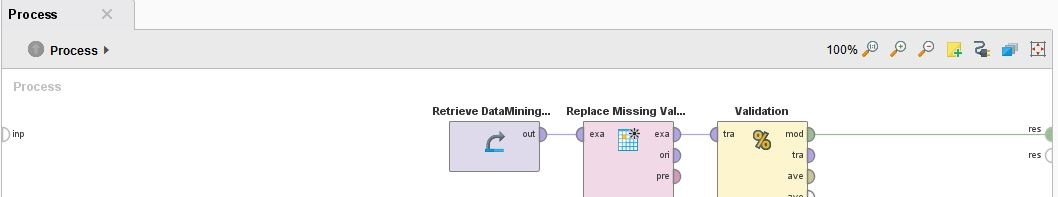
\includegraphics[width=\linewidth]{1.jpg}
  \caption{}
    \label{tab:example}
\end{figure}
\begin{figure}[!h]
  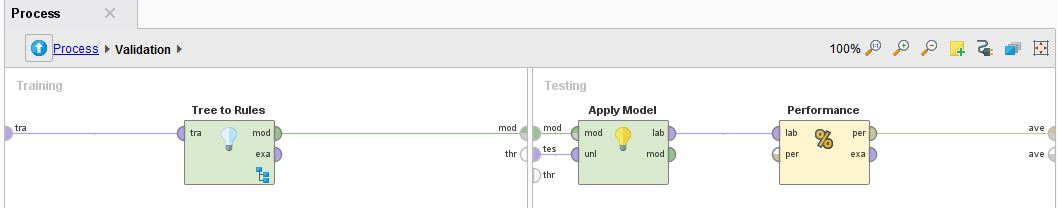
\includegraphics[width=\linewidth]{2.jpg}
    \caption{}
    \label{tab:example}
\end{figure}
\begin{figure}[!h]
  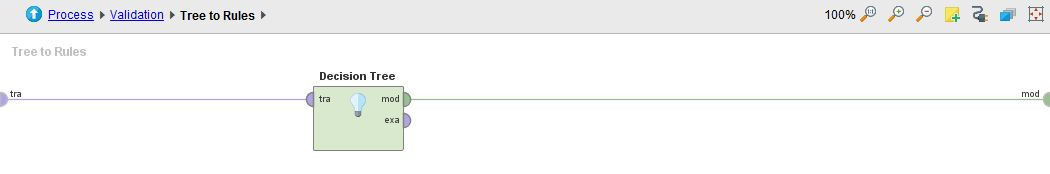
\includegraphics[width=\linewidth]{3.jpg}
    \caption{}
    \label{tab:example}
\end{figure}

\newpage
\subsection{بدست آوردن قانون‌ها از درخت \lr{Cart}}
\paragraph{}
در این روش، تمامی مراحل شبیه به روش قبل است. نیازی به تبدیل داده‌ها به داده‌های عددی نیست و جهت یادگیری و تست از ماژول \lr{Validation} استفاده می‌شود. همچنین از ماژول \lr{Tree to Rule} جهت بدست آوردن قوانین استفاده می‌کنیم. تنها تفاوت این روش با درخت \lr{ID3} در این است که معیار ماژول \lr{Decision tree} را بروی \lr{Gini Index} میگذاریم.


تذکر: ما ترجیح دادیم که برای پیاده‌سازی و استخراج قوانین از ماژول‌های استاندارد \lr{RapidMiner} استفاده کنیم. ضمن اینکه می‌توان با دانلود افزونه \lr{Weka} و استفاده از ماژول‌های آن، نتیجه‌های دیگری گرفت. اگرچه می‌توانستیم ولی از نظر ما ماژول \lr{RapidMiner} دقت بهتری داشت.


\subsection{الگورتیم \lr{KNN}}
\paragraph{}
این الگوریتم بروی داده‌های عددی قابل پیاده‌سازی است. بنابراین با استفاده از ماژول \lr{Nominal to Numerical} داده‌ها به عدد تنظیم می‌کنیم. هم‌چنین جهت تبدیل از روش \lr{Unique Integer} استفاده می‌کنیم به این معنا که به هر حرف یک عدد خاص نسبت میدهد.
سپس ماژول \lr{Validation} را جهت انجام یادگیری و تست انتخاب می‌کنیم و ماژول \lr{k-NN} را در این قسمت قرار میدهیم. همچنین مقدار \lr{K} را بروی 3 قرار می‌دهیم تا برای هر پیش‌بینی از 3 همسایه نزدیک استفاده کند. ضمن اینکه نوع اندازه‌گیری را بروی \lr{NumericalMeasure} قرار داده و از فاصله اقلیدسی جهت محاسبه فاصله‌ها استفاده می‌کنیم.



\end{document}